\section{DnsCompression}\label{sec:dnscomp}

\begin{figure}
\begin{center}
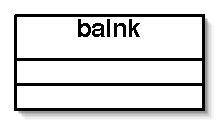
\includegraphics[width=0.4\textwidth]{figs/blank}
\end{center}
\caption{}
\label{fig:dnscomp}
\end{figure}

This section describes the DnsCompression component, which is described by Figure~\ref{fig:blank}.

DNS name compression is tricky business, and this class aims to simplify it by providing a compression context.

\subsection{Methods}

{\bf Public Methods}
\begin{itemize}
\item add\_name(): This method takes a name and returns the number of leading name parts that remain after compression. It also returns a pointer if any compression occurs. It records metadata for use in future add\_name() method calls.
\end{itemize}

\subsection{Member Variables}
\begin{itemize}
\item m\_names: A mapping of names and sub-names to DNS pointers. For the purposes of compression, the names are actually stored backwards.
\end{itemize}
